\documentclass[10pt,twocolumn]{article}

% use the oxycomps style file
\usepackage{oxycomps}

% usage: \fixme[comments describing issue]{text to be fixed}
% define \fixme as not doing anything special
\newcommand{\fixme}[2][]{#2}
% overwrite it so it shows up as red
\renewcommand{\fixme}[2][]{\textcolor{red}{#2}}
% overwrite it again so related text shows as footnotes
%\renewcommand{\fixme}[2][]{\textcolor{red}{#2\footnote{#1}}}

% read references.bib for the bibtex data
\bibliography{references.bib}

% include metadata in the generated pdf file
\pdfinfo{
    /Title (Reference-Free Evaluation Framework for Stem Separation)
    /Author (Jiayi Wang)
}

% set the title and author information
\title{Reference-Free Evaluation Framework for Stem Separation}
\author{Jiayi Wang}
\affiliation{Occidental College}
\email{jwang2@oxy.edu}

\begin{document}

\maketitle

\section{Introduction}
Audio source separation is a critical task in the field of audio signal processing, with applications spanning music production, audio restoration, and automatic transcription. Recent advances in deep learning have enabled substantial progress in separating complex audio mixtures into their constituent stems, such as vocals, drums, bass, and others. However, evaluating the quality of separated audio stems requires the ground truth for individual stems, which is not always accessible from a consumer's standpoint. Also, traditional metrics like Signal-to-Distortion Ratio (SDR), Signal-to-Interference Ratio (SIR), and Signal-to-Artifact Ratio (SAR) provide valuable insights into separation quality but are limited in capturing nuanced aspects such as harmonic integrity and temporal stability.

The effectiveness of a stem separation algorithm depends not only on its ability to suppress interference and artifacts but also on how well it preserves the spectral and dynamic characteristics of the original stems. Harmonic content must be retained for musical instruments to sound natural, and the temporal stability of energy must be maintained to ensure the separation is perceptually coherent. These requirements highlight the need for complementary evaluation metrics that extend beyond the scope of traditional measures.

To address these challenges, we propose a reference-free evaluation framework that introduces two novel metrics: the Frequency Isolation Score (FIS) and the Dynamic Stability Score (DSS). FIS measures the effectiveness of frequency isolation and harmonic preservation, while DSS assesses temporal energy consistency and spectral flux stability. Together, these metrics aim to provide a multidimensional perspective on separation quality, complementing traditional measures like SAR.

This paper is structured as providing a technical background on the key methods and algorithms used in source separation and reviewing prior work in the field, focusing on existing evaluation approaches. Methods section details the proposed metrics and methodologies, including their theoretical foundations and implementation. Then this study presents the evaluation results, followed by a discussion of their implications. The paper concludes with ethical considerations, future directions, and code documentation.

By introducing FIS and DSS, this study aims to advance the field of audio source separation by providing a comprehensive evaluation framework that addresses the limitations of traditional metrics while paving the way for future innovations in audio quality assessment.

\section{Technical Background}

Audio source separation relies on advanced signal processing techniques and algorithms designed to isolate individual components, or "stems," from complex audio mixtures. This section introduces the key technical concepts underlying the proposed evaluation framework, including the spectrogram, Short-Time Fourier Transform (STFT), and an overview of current state-of-the-art stem separation algorithms.

\subsection{Spectrogram and Short-Time Fourier Transform}

The spectrogram is a widely used tool in audio analysis, representing the frequency content of a signal as a function of time. It is generated by applying the Short-Time Fourier Transform (STFT), which decomposes a time-domain signal into overlapping time-frequency bins. The STFT is defined as:

\[
X(t, \omega) = \sum_{n=-\infty}^{\infty} x[n] w[n-t] e^{-j \omega n}
\]

Where:
\begin{itemize}
    \item \(X(t, \omega)\) represents the complex STFT coefficients, providing both magnitude and phase information at each time-frequency bin.
    \item \(x[n]\) is the discrete time-domain audio signal.
    \item \(w[n-t]\) is the window function, typically a Hamming or Hann window, used to segment the signal into overlapping frames.
    \item \(e^{-j \omega n}\) is the Fourier kernel, enabling the transformation from the time domain to the frequency domain.
\end{itemize}


\subsection{Spectrogram Visualization}
The spectrogram is obtained by plotting the magnitude of the STFT coefficients (\(|X(t, \omega)|\)). This representation provides a detailed view of the harmonic and transient structures within an audio signal.

To illustrate the time-frequency representation used in stem separation, Figure~\ref{fig:spectrogram_full} shows the spectrogram of an audio mix, while Figure~\ref{fig:spectrogram_stem} depicts the spectrogram of an isolated vocal stem obtained through separation. The x-axis represents time in seconds, while the y-axis represents frequency in Hertz (Hz). The color intensity indicates the magnitude of the spectral content, with brighter regions corresponding to higher energy at specific frequencies and times.

\begin{figure}[h]
    \centering
    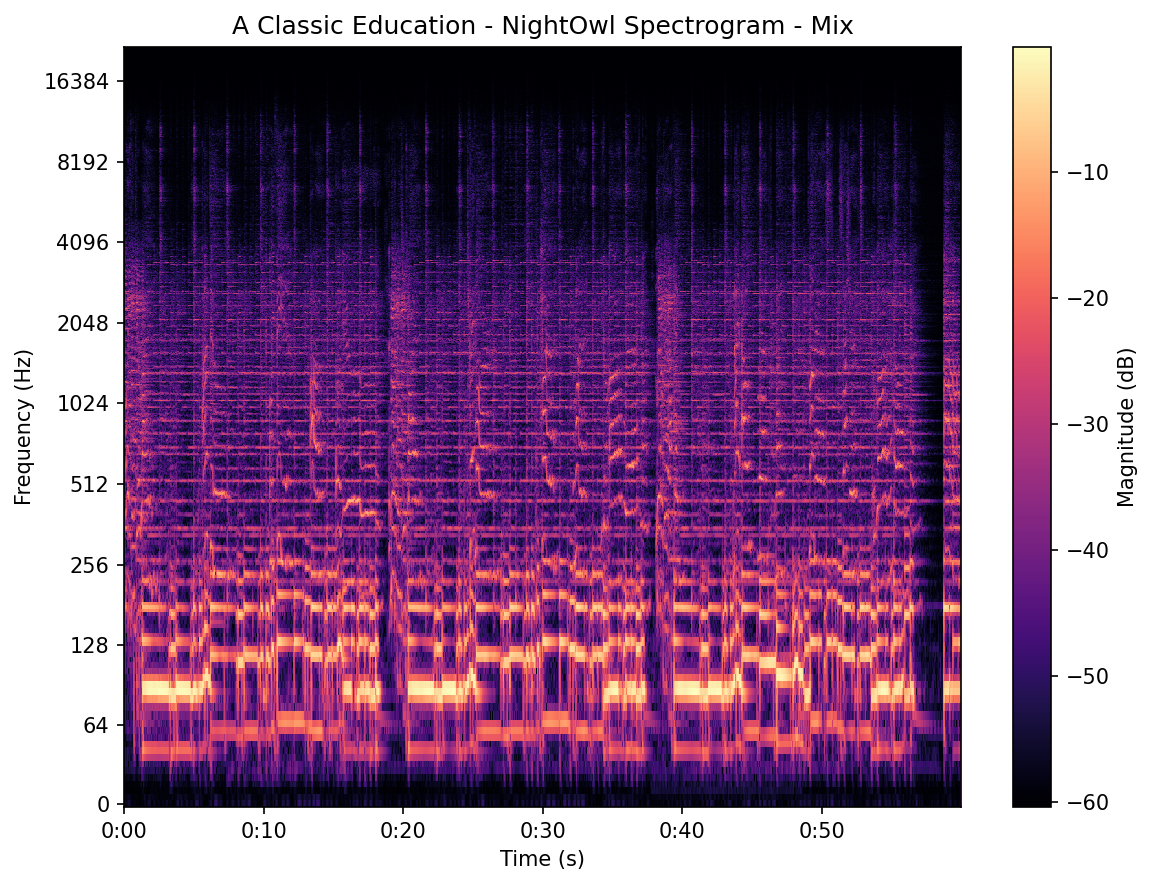
\includegraphics[width=0.95\linewidth]{results graph/mix.png}
    \caption{Spectrogram of the complete audio mix. The dense frequency content represents the overlap of various stems, including vocals, instruments, and noise.}
    \label{fig:spectrogram_full}
\end{figure}

The spectrogram of the isolated stem (Figure~\ref{fig:spectrogram_stem}) demonstrates how the stem separation process reduces interference and preserves harmonic content. For example, the fundamental frequency of the vocal line and its harmonics are clearly visible, while unrelated frequencies from other stems are suppressed.

\begin{figure}[h]
    \centering
    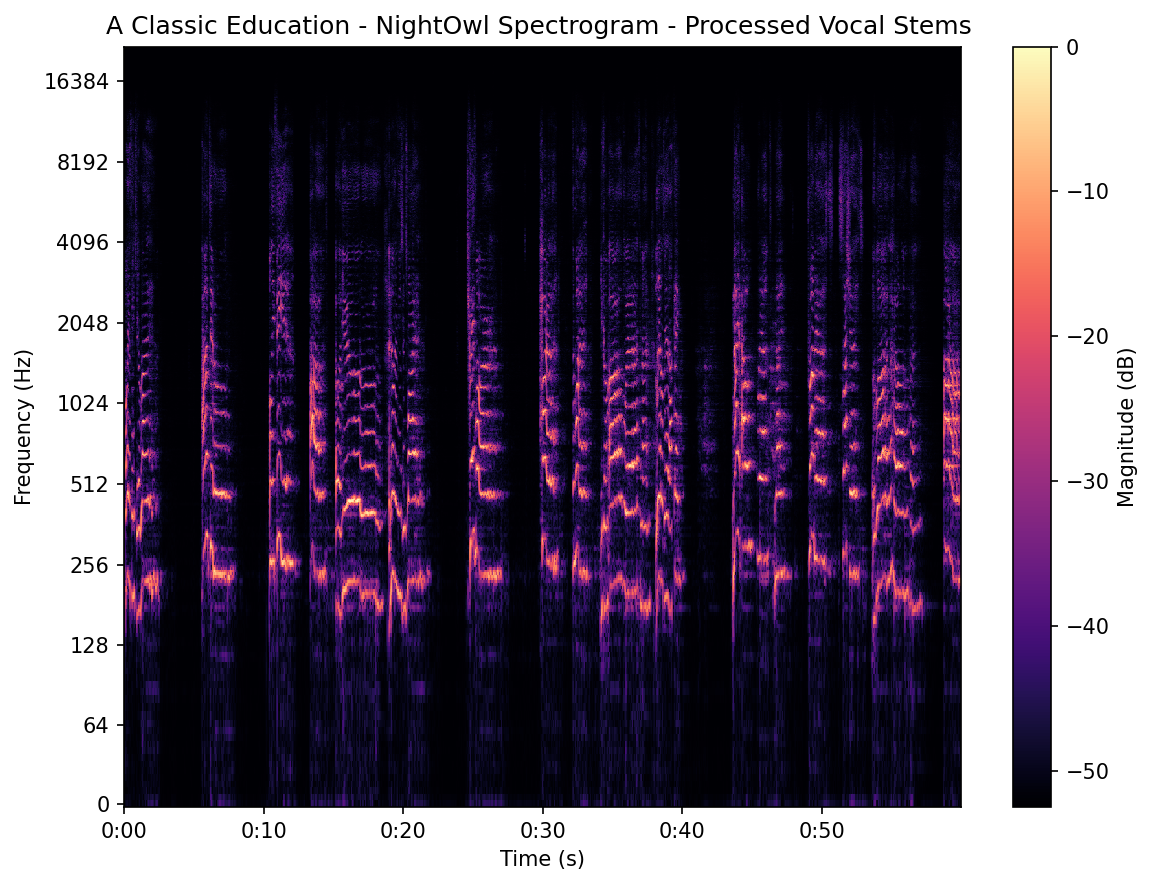
\includegraphics[width=0.95\linewidth]{results graph/vocal.png}
    \caption{Spectrogram of an isolated vocal stem. Harmonics of the fundamental frequency are preserved, while interference from other stems is minimized.}
    \label{fig:spectrogram_stem}
\end{figure}

\subsection{Stem Separation Algorithms}

Recent advancements in machine learning and signal processing have led to the development of algorithms for audio stem separation. These methods can be categorized into time-domain and frequency-domain approaches:

\subsubsection{Time-Domain Algorithms}
Time-domain methods operate on the raw audio waveform, leveraging deep learning models to predict individual stems. \textbf{Demucs} employs recurrent neural networks to achieve high-quality separation. By avoiding the need for explicit time-frequency transformations, time-domain models maintain phase coherence and exhibit robust temporal performance.

\subsubsection{Frequency-Domain Algorithms}
Frequency-domain methods operate on the spectrogram, leveraging the rich time-frequency representation to isolate stems. \textbf{Open-Unmix (UMX)} utilizes deep learning to separate stems by analyzing spectral patterns. Frequency-domain approaches excel in capturing harmonic relationships and are effective for instruments with distinct spectral characteristics.

\section{Prior Work}

The field of audio source separation has seen advancements, with contributions to both algorithm and evaluation methodologies. Early works, such as Vincent et al.~\cite{vincent2006}, laid the foundation for performance measurement in blind source separation, introducing metrics like Signal-to-Distortion Ratio (SDR), Signal-to-Interference Ratio (SIR), and Signal-to-Artifact Ratio (SAR). These metrics have since become the standard for evaluating separation quality in benchmark campaigns like SiSEC~\cite{araki2011, stoter2018}.

Recent efforts have explored perceptual and referenceless evaluation methods. Cano et al.~\cite{cano2016} highlighted the gap between human perception and quantitative metrics, advocating for metrics that better align with subjective quality assessments. Similarly, Grais et al.~\cite{grais2018} proposed a referenceless evaluation framework leveraging deep learning, while Simpson et al.~\cite{simpson2017} emphasized the importance of psychophysical testing in assessing separation performance.

Despite these advancements, traditional metrics like SDR and SAR remain widely used due to their simplicity and computational efficiency~\cite{roux2019}. This study contributes to this field of literature by proposing a reference-free evaluation framework that emphasizes the signal processing characteristics of stem separation. Unlike traditional metrics such as SAR, which require access to ground truth reference stems, my approach operates independently of such references, making it applicable to scenarios where references are unavailable. Existing reference-less evaluation methods, such as those based on deep learning, often focus on perceptual alignment rather than the core signal processing aspects of the task. Similarly, while human listening tests provide valuable insights, they are subjective, time-consuming, and impractical for large-scale evaluation. In contrast, the proposed metrics are rooted in signal processing principles, offering an objective, automated, and scalable solution that evaluates separation quality based on frequency isolation and temporal stability, two fundamental aspects of audio signal separation.

\section{Methods}
This section introduces the proposed reference-free evaluation framework for audio stem separation, focusing on two metrics: the Frequency Isolation Score (FIS) and the Dynamic Stability Score (DSS). These metrics are designed to assess key aspects of separation quality, specifically frequency isolation and temporal stability, without relying on reference ground truth stems. By leveraging signal processing techniques, the proposed framework provides an objective and scalable approach to evaluating separation performance, addressing the limitations of both traditional metrics and existing reference-less methods. .

\subsection{Frequency Isolation Score(FIS)}

The Frequency Isolation Score (FIS) is designed to measure the effectiveness of frequency isolation for a given stem within a mix, focusing on the presence of the fundamental frequency and harmonics. This score helps to evaluate how well the stem is separated from the mix, preserving its key frequency content while ensuring that harmonic components are properly retained. The FIS is intended to assess the isolated stem's quality on a scale ranging from 0 to 100, where higher scores represent better isolation and frequency preservation.

The FIS evaluation consists of two main components:
\begin{itemize}
    \item Fundamental Frequency Score: Evaluates the presence of the fundamental frequency of the stem in the mix, contributing a fixed 40 points if present.
    \item Harmonics score: Evaluates the presence of harmonic frequencies in the mix, contributing up to 60 points based on how well the harmonic frequencies are preserved in comparison to the stem.
\end{itemize}

This algorithm starts by performing the Short-Time Fourier Transform (STFT) on both mixed audio and individual stems. After performing the Short-Time Fourier Transform (STFT) on the stem, we proceed by analyzing the resulting frequency components to identify the fundamental frequency. The fundamental frequency of the stem is identified by detecting the index of the lowest frequency component with nonzero energy in the stem's STFT representation. Mathematically, the fundamental frequency can be detected as follows:

\[
f_0 = arg min_{f} {|X(f, t)| > 0}
\]

Where:

\begin{itemize}
    \item \(f_0 \) is the fundamental frequency.
    \item \(X(f, t) \) is the STFT magnitude of the signal at frequency f and time t.
    \item \(arg min_{f} \) denotes the frequency index at which the magnitude is non-zero and the lowest.
\end{itemize}


If the same fundamental frequency is present in the mix, a fixed 40 points are awarded to indicate that the most significant tonal component of the instrument. The fundamental frequency is crucial in maintaining the integrity of the stem's identity, as it is the primary building block of the harmonic structure. This fixed score ensures that the presence of the fundamental tone is prioritized. Thus, detecting the fundamental frequency in the mix is considered a baseline requirement for effective isolation, contributing a stable 40 points to the overall score, regardless of the performance of higher harmonics.

After identifying the fundamental frequency, the next step is to locate the harmonic frequencies of the stem. The harmonics, along with the fundamental frequency, define the characteristic sound of an instrument, and their accurate isolation is essential for high-quality stem separation. Harmonics are integer multiples of the fundamental frequency and are key components that contribute to the timbre and richness of the sound. By finding and analyzing these harmonics, we can evaluate how well the harmonic content of the stem is preserved in the mix. Thus, finding the harmonic indices is crucial for understanding the fidelity of the stem's harmonic structure in the separation process. The harmonic indices are calculated as:

\[
\text{Harmonic Indices} = f_0 \times (n + 1), \quad \text{for } n = 1, 2, 3, \ldots, N
\]
Where \(f_0\) is the fundamental frequency index and \(N\) is the maximum number of harmonics such that the harmonic frequency does not exceed 20,000 Hz.

\vspace{0.5cm}

The harmonic frequencies are calculated as:
\[
f_{\text{harmonic}} = f_0 \cdot (k + 1), \quad \text{for } k = 1, 2, 3, \ldots, K
\]
Where \(f_0\) is the fundamental frequency and \(K\) is the number of harmonics such that \(f_{\text{harmonic}} \leq 20,000\) Hz.

\vspace{0.5cm}

After getting the fundamental and harmonic information, The final Frequency Isolation Score (FIS) is calculated as:
\[
S_{\text{FIS}} = S_{\text{fundamental}} + S_{\text{harmonics}}
\]
Where:
\begin{itemize}
  \item \(S_{\text{fundamental}}\) is the fixed score of 40 if the fundamental is present.
  \item \(S_{\text{harmonics}}\) is the normalized score (out of 60) based on the presence of harmonics in the mix.
\end{itemize}
\subsection{Dynamic Stability Score(DSS)}
The Dynamic Stability Score (DSS) is designed to evaluate the temporal energy stability of a given stem within a mix, focusing on the consistency of the stem's dynamic profile and the changes in spectral content over time. This score helps in assessing how stable the energy of the isolated stem remains, indicating whether the instrument has been effectively separated while maintaining a consistent dynamic behavior. The DSS is intended to measure stability, where higher scores indicate greater dynamic consistency and fewer unwanted fluctuations. The DSS evaluation consists of two main components:
\begin{itemize}
    \item Dynamic Stability Score (DSS): Assesses the stability of the stem's RMS energy levels by evaluating the mean to standard deviation ratio of active frames, which contributes significantly to the final score.
    \item Spectral Flux Score: Measures the rate of change in spectral content between consecutive frames. A higher flux indicates instability, and therefore contributes a penalty to the overall score.
\end{itemize}


The \textit{Dynamic Stability Score (DSS)} is calculated to evaluate how stable the energy level of a stem is over time. We utilize the Root Mean Square (RMS) energy values to determine the consistency of the signal.
The \textit{Root Mean Square (RMS)} is a statistical measure used to calculate the magnitude of a varying signal over time. For a discrete signal \( x[n] \) consisting of \( N \) samples, the RMS value can be computed as follows:

\begin{equation}
    \text{RMS} = \sqrt{\frac{1}{N} \sum_{n=1}^{N} x[n]^2}
\end{equation}

Where:
\begin{itemize}
    \item \( x[n] \) represents the amplitude of the signal at sample \( n \).
    \item \( N \) is the total number of samples.
\end{itemize}

The RMS values provide a measure of the signal's energy across different frames. Using these RMS values, we can determine the consistency of the energy in the stem, which forms the basis for calculating the Dynamic Stability Score (DSS). The DSS is defined as:

\begin{equation}
    \text{DSS} = \frac{\mu_{\text{RMS}}}{\sigma_{\text{RMS}} + \epsilon}
\end{equation}

Where:
\begin{itemize}
    \item $\mu_{\text{RMS}}$ is the mean RMS value of the active frames in the stem signal.
    \item $\sigma_{\text{RMS}}$ is the standard deviation of the RMS values of the active frames.
    \item $\epsilon$ is a small constant ($1 \times 10^{-6}$) added to avoid division by zero.
\end{itemize}



In addition to evaluating energy consistency using the Dynamic Stability Score (DSS), we also consider the variation in the spectral content over time to assess the overall stability of the stem. This variation is measured by the \textit{Spectral Flux}, which quantifies the rate of change in the spectral content of the stem signal across consecutive time frames. It is defined as:

\begin{equation}
    \Delta(t) = \sum_{f=1}^{F} \left( |X(f, t+1)| - |X(f, t)| \right)^2
\end{equation}

Where:
\begin{itemize}
    \item $X(f, t)$ represents the magnitude of frequency bin $f$ at time frame $t$.
    \item $\Delta(t)$ represents the flux difference between consecutive frames.
    \item $F$ is the total number of frequency bins.
\end{itemize}


The final dynamic stability score is computed by combining the DSS and the Spectral Flux penalty:

\begin{equation}
    \text{Final Score} = \text{DSS}_{\text{normalized}} - \text{Flux Score} 
\end{equation}

Where:
\begin{itemize}
    \item $\text{Baseline}$ is set to $20$.
    \item $\text{DSS}_{\text{normalized}}$ and $\text{Flux Score}$ are calculated as described in previous sections.
\end{itemize}

\textit{Spectral Flux} is not suitable for evaluating inherently dynamic instruments like drums. For such instruments, we set the \textit{Flux Score} to $0$ to avoid unfair penalties due to high flux variability. This is a necessary adjustment to prevent skewed evaluations.
The dynamic stability evaluation framework provides a comprehensive method to assess the quality of stem separation by accounting for both energy stability and spectral changes. While this approach works well for most instruments, modifications are necessary for instruments with inherently high variability, such as drums.

\section{Evaluation Metrics}
To evaluate the performance of audio stem separation algorithms, we focused on Signal-to-Artifact Ratio (SAR) as the primary metric. SAR was selected because it combines the scores between Signal-to-Distortion Ratio (SDR) and Signal -to-interference Ratio (SIR). While SIR typically measures interference suppression, it demonstrated near-perfect scores across the entire dataset in this study. This result in SDR and SAR to be the same value. As such, SIR and SDR were excluded from further analysis, and the evaluation centered on SAR in conjunction with the proposed metrics: Frequency Isolation Score (FIS) and Dynamic Stability Score (DSS).

Two statistical methods were employed to evaluate the relationships between SAR, FIS, and DSS: Pearson correlation and linear regression. Pearson correlation was used to quantify the linear relationships between SAR and the proposed metrics individually. This method determine whether changes in one metric correspond to changes in another. Linear regression was employed to model SAR as a function of FIS and DSS. 

\subsection{Dataset}
The dataset used for this evaluation is the MUSDB18-HQ\cite{musdb18-hq} in its uncompressed format, a widely recognized dataset for audio source separation tasks. MUSDB18-HQ provides high-quality ground truth stems for various tracks, allowing accurate evaluation of separation algorithms. Each track in the dataset was separated into four stems: vocals, drums, bass, and other.

For this study, we applied source separation using two state-of-the-art algorithms:
\begin{itemize}
    \item Demucs: A time-domain algorithm designed for high-quality stem separation, leveraging deep learning to enhance temporal consistency.
    UMX (Open-Unmix): A frequency-domain method that isolates stems by analyzing spectral content, optimizing for harmonic separation.
\end{itemize}  

The algorithms were evaluated on the MUSDB18-HQ dataset to ensure a consistent and reliable comparison. Both SAR and the proposed metrics, FIS and DSS, were calculated for each of the four stems across all tracks, enabling a comprehensive assessment of separation performance.

\section{Evaluation Results and Discussion}

\subsection{Correlation Analysis}
Pearson correlation analysis was conducted to examine the linear relationships between Signal-to-Artifact Ratio (SAR) and the proposed metrics: Frequency Isolation Score (FIS) and Dynamic Stability Score (DSS). The results revealed a weak negative correlation between SAR and FIS, with a Pearson correlation coefficient of $r = -0.17$. This suggests that higher frequency isolation may slightly increase artifacts, leading to lower SAR values. In contrast, SAR and DSS showed a weak positive correlation, with $r = 0.18$, indicating that greater temporal stability is marginally associated with better artifact suppression.

These weak correlations highlight the distinct evaluation dimensions of the metrics. While SAR primarily measures artifact suppression, FIS focuses on frequency-domain isolation, and DSS captures temporal consistency. The limited alignment between these metrics underscores their potential to provide complementary insights into separation quality rather than overlapping perspectives.
\begin{figure}
    \centering
    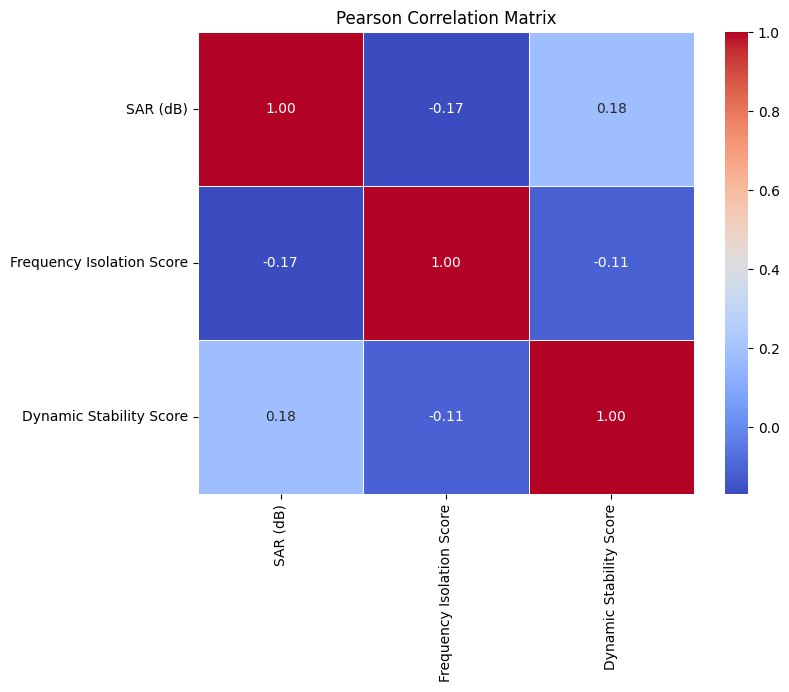
\includegraphics[width=.95\linewidth]{results graph/Pearson Correlation Matrix.png}
    \caption{
        Pearson Correlation Matrix
    }
    \label{fig:first-page}
\end{figure}
\subsection{Regression Analysis}
Multiple linear regression was performed to assess the combined and individual effects of FIS and DSS on SAR. The regression model achieved an $R^2$ value of $0.055$, indicating that only 5.5\% of the variance in SAR could be explained by FIS and DSS. The adjusted $R^2$ was $0.043$, accounting for the number of predictors. Despite the low explanatory power, the model’s F-statistic of $F = 4.46$ with a $p$-value of $0.013$ indicated that FIS and DSS jointly had a statistically significant effect on SAR.

The regression coefficients revealed further insights into the relationships. The intercept was $8.68$, representing the baseline SAR when both FIS and DSS were zero. The coefficient for FIS was $-0.0488$, suggesting that for every unit increase in frequency isolation, SAR decreases slightly by approximately $0.049$. Conversely, the coefficient for DSS was $0.0287$, indicating a minor positive effect on SAR, with each unit increase in temporal stability resulting in a $0.029$ increase in SAR. These findings suggest that while FIS and DSS together influence SAR, their individual effects are modest.
\begin{figure}
    \centering
    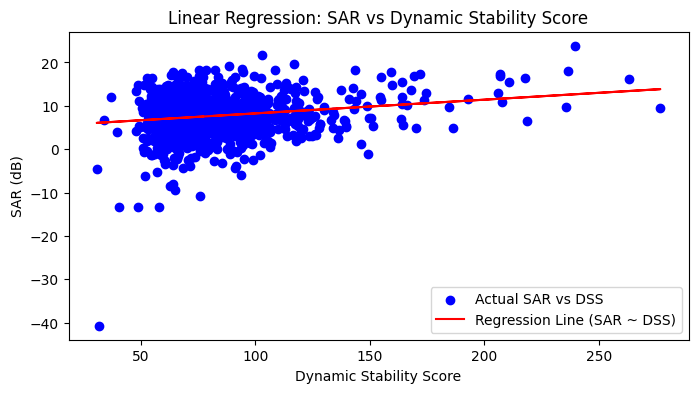
\includegraphics[width=.95\linewidth]{results graph/Linear Regression SAR vs DSS.png}
    \caption{
        Linear Regression SAR vs DSS
    }
    \label{fig:first-page}
\end{figure}
\begin{figure}
    \centering
    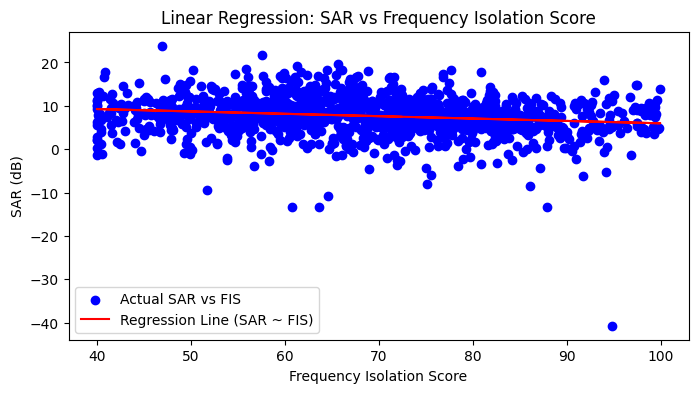
\includegraphics[width=.95\linewidth]{results graph/Linear regression SAR vs FIS.png}
    \caption{
        Linear Regression SAR vs FIS
    }
    \label{fig:first-page}
\end{figure}
\subsection{Discussion}

The results underscore the roles of SAR, FIS, and DSS in evaluating audio separation quality. The weak correlations between SAR and the proposed metrics reflect their different scopes. SAR evaluates artifact suppression, while FIS measures frequency isolation, and DSS assesses temporal consistency. These differences explain the limited alignment observed in correlation analysis but also highlight the potential of FIS and DSS to complement SAR in a multidimensional evaluation framework.

The regression analysis supports these observations, demonstrating that while FIS and DSS jointly influence SAR, their explanatory power is limited. The weak negative relationship between FIS and SAR suggests a potential trade-off, where improving frequency isolation may increase artifacts, thus reducing SAR. In contrast, the weak positive relationship between DSS and SAR indicates that a higher temporal stability aligns slightly with improved artifact quality. However, the low $R^2$ score of the regression model suggests that SAR is influenced by additional factors not captured by FIS and DSS, pointing to the need for a broader evaluation framework.

From a practical perspective, these findings demonstrate the value of FIS and DSS as complementary metrics. Although SAR remains essential for assessing artifact suppression, FIS and DSS provide valuable insights into frequency domain and temporal aspects of separation quality. Together, these metrics enable a more nuanced evaluation of separation algorithms, aligning with specific application priorities. Future work should focus on integrating perceptual evaluation methods and developing new metrics to bridge the gap between artifact suppression, frequency isolation, and temporal stability.

\section{Ethical Considerations}

The proposed reference-free evaluation framework is designed to objectively assess the quality of audio stem separation algorithms, but it is essential to address potential ethical implications. One key consideration is the responsible use of these metrics in applications such as music production, copyright analysis, and audio forensics. Ensuring that these tools are not misused to infringe on intellectual property rights or to bypass licensing agreements is critical to maintaining ethical integrity.

The automation of audio quality assessment through signal processing metrics like FIS and DSS reduces reliance on human evaluators. While this enhances scalability and objectivity, it also raises concerns about potential biases encoded in the metrics themselves. To mitigate this, the framework was developed with a focus on signal fidelity and temporal consistency, avoiding reliance on subjective or culturally biased criteria.

Furthermore, the framework's potential applications in training and evaluating machine learning models must be approached with caution. Developers should ensure that these models do not perpetuate or amplify existing inequalities in access to music production tools or inadvertently prioritize certain genres or musical styles due to biases in evaluation criteria. Transparency in reporting metric performance and limitations is crucial to fostering trust and accountability.

Finally, it is important to respect the privacy and consent of individuals when using separated stems for research or application purposes. Datasets such as MUSDB18-HQ~\cite{musdb18-hq} are invaluable for evaluating separation algorithms, but their use should always adhere to licensing terms and ethical guidelines. By addressing these considerations, this framework aims to contribute to the advancement of audio separation research while promoting responsible and ethical practices.
\section{Future Work and Conclusion}

The proposed reference-free evaluation framework provides a novel approach to assessing audio stem separation quality by focusing on signal processing attributes such as frequency isolation and temporal stability. Its design eliminates the reliance on ground truth references, making it suitable for evaluating AI-generated music stems, where no definitive ground truth exists. This capability is crucial as AI systems increasingly generate music content that deviates from traditional recording paradigms, requiring new evaluation standards to ensure quality and usability.

Future research could explore the relationship between AI-generated separated stems and those produced by human-engineered separation techniques. Such studies could evaluate whether AI-generated stems exhibit comparable levels of fidelity, harmonic preservation, and temporal consistency, and assess the practical applicability of these stems in real-world audio production contexts. Additionally, integrating perceptual evaluation with the proposed metrics could further bridge the gap between signal processing quality and listener satisfaction, providing a more holistic assessment framework.

In conclusion, the Frequency Isolation Score (FIS) and Dynamic Stability Score (DSS) offer a robust and scalable solution to the challenges of stem separation evaluation. By addressing limitations of traditional and existing referenceless methods, this framework lays the foundation for broader applications in music production, AI-generated audio content, and automated assessment of audio quality. Future advancements in this area will continue to enhance the objectivity, efficiency, and applicability of evaluation methods, driving innovation in audio signal processing and music technology.


\section{Code Documentation}

\subsection{Replication Instructions}

To replicate the proposed evaluation framework, follow these steps:

\textbf{1. Dependencies:}
\begin{itemize}
    \item Python 3.8 or higher.
    \item Required libraries:
    \begin{itemize}
        \item \texttt{librosa}: For audio processing and spectral analysis.
        \item \texttt{numpy}: For numerical computations.
        \item \texttt{matplotlib}: For visualizations.
        \item \texttt{mir\_eval}: For traditional metric calculations.
        \item \texttt{openunmix}: For source separation tasks.
        \item \texttt{demucs}: For time-domain stem separation.
    \end{itemize}
    \item Additional tools: FFmpeg (optional, for audio conversion if needed).
\end{itemize}

\textbf{2. Dataset Setup:}
\begin{itemize}
    \item Obtain the MUSDB18-HQ dataset~\cite{musdb18-hq} from its official source.
    \item Extract the dataset into a folder named \texttt{data/musdb18hq/}, ensuring it contains subfolders for each track with stems such as \texttt{vocals}, \texttt{bass}, \texttt{drums}, and \texttt{other}.
\end{itemize}

\subsection{Code Architecture Overview}

 The structure is as follows:

\begin{verbatim}
code/
  analysis/
    Analysis.ipynb
    evaluate.py 
    sap.py
  scores/
    Dynamic_Stability_Score.py           
    Frequency_Isolation_Score.py
    score.py
evaluation_results/
  evaluation_graphs/
    Linear Regresion SAR vs DSS.png 
    Linear Regresion SAR vs FIS.png 
    Pearson Correlation Metrics.png
  CSV/
    evaluation_results.csv
logs/
    evaluation_log.txt
    sap_log.txt
    umx_log.txt
README.md
\end{verbatim}

\textbf{Folder Descriptions:}
The \texttt{analysis/} folder contains scripts and notebooks for orchestrating the evaluation process. The \texttt{Analysis.ipynb} notebook is for generating graphs for analysis, while \texttt{evaluate.py} generates all CSV files. The \texttt{sap.py} script is used for preprocessing and handling source separation outputs.

The \texttt{scores/} folder includes scripts implementing the proposed metrics. \texttt{Frequency\_Isolation\_Score.py} computes the FIS metric, while \texttt{Dynamic\_Stability\_Score.py} calculates the DSS metric. The \texttt{score.py} script is the code for generating scores from the functions above.

The \texttt{evaluation\_results/} folder organizes the outputs of the evaluation process. The \texttt{evaluation\_graphs/} subfolder contains visualizations such as regression plots and correlation matrices, while the \texttt{CSV/} subfolder stores summarized results in \texttt{evaluation\_results.csv}.

Finally, the \texttt{logs/} folder tracks the evaluation process, storing runtime details in \texttt{evaluation\_log.txt} and specific logs for source separation models like UMX (\texttt{umx\_log.txt}) and SAP (\texttt{sap\_log.txt}). The \texttt{README.md} file provides an overview of the project and instructions for running the framework.


\printbibliography

\end{document}
